\chapter{Numerical Simulations of Stenotic Flow}

Peripheral arterial occlusive diseases, especially in femoral arteries are commonly seen by clinical doctors in the U.S.\cite{malinow1989prevalence, boger1997biochemical, hooi2001incidence}. These patients may have critical stenoses or multiple sequential moderate stenoses. The current clinical practice usually recommends simple balloon angioplasty\cite{duncan1995simple} to treat critical stenotic lesion, i.e. $ > 60 \% $ luminal area reduction. However, it is a difficult process for the doctors to make a decision on whether or not to treat multiple sequential moderate stenoses using the stent or balloon angioplasty. This is partially because of the lack of methods to measure how these multiple stenoses affect their downstream blood flow. The scientific study of fluid dynamics associated with multiple stenoses is far less than that of a single stenosis. To assist on making clinical decision for treating multiple stenoses, a quantitative approach, for instance, the computational fluid dynamics (CFD) \cite{ferziger1997computational} method is very much needed. In this study,  we present a high-fidelity CFD simulations of the blood flow in the stenotic arteries using idealized geometries. We solve unsteady incompressible Navier-Stokes equations\cite{temam1984navier} using unstructured meshes with all hexahedral elements. The upstream flow condition is prescribed which gives a Reynolds number of 500. Our simulations results reveal several new discoveries of fluid dynamics in these multiple stenoses considering a range of different geometric parameters.

\section{Background}

Peripheral arterial occlusive disease are the major cause of amputation in the U.S. as they are prevalent among smokers, diabetics, hypertensives, and patients with dyslipidemia. Nowadays, since the disease can be visualized as areas of stenosis or occlusion on a diagnostic arteriogram, simple balloon angioplasty with or without stenting is usually recommended for treating critical stenotic lesions, i.e. $ > 60\% $ (by area) luminal reduction. However, the clinical decision is rather difficult on whether or not to treat subcritical stenotic lesions, i.e., $ < 50\% $ luminal reduction, in particular, multiple sequential moderate stenoses. The risks of routine ballloon angioplasty/stenting include intimal injury-induced acute arterial thrombosis or restenosis\cite{holmes1984restenosis} from neointimal hyperplasia\cite{kornowski1998stent}, etc. These risks led to the difficulty of telling the benefits of treating mildly stenotic lesions using routine clinical treatment. Meanwhile, there is no existing method to measure the effects of multiple sequential moderate stenoses on blood flow in the part of the artery that is downstream of the stenotic lesions. The closest measurement that correlated with change in blood flow is the change in arterial pressures. If the arterial pressure drop across the stenoses is greater than the clinical threshold (20-30mmHg) \cite{meuwissen2002hyperemic}, the lesions are considered physiologically significant enough to favor treatment. However, it's clinically very difficult to quantify. Consequently, CFD simulation is a helpful supplement for the stenosis study.

\begin{figure}[H]
	\centering
	\begin{tabular}{c}
		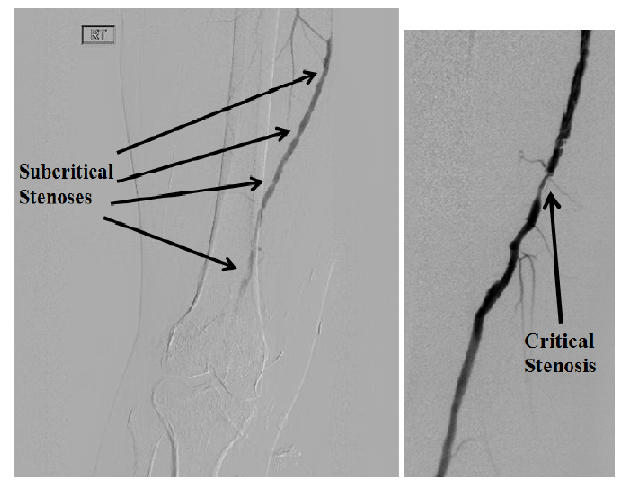
\includegraphics[width=0.6\textwidth]{./pics/photo.png}
	\end{tabular}
	\caption{\footnotesize Contrast of subcritical and critical stenoses.}
\end{figure}

A good amount of investigation have been addressed on pressure drop across single stenosis from both experimental and analytical perspective\cite{Ojha,Varghese,Young&Tsai,Young&Cholvin,Seeley&Young,Varghese&Frankel}. At the beginning, investigators derived empirical function from conservation equations with the experimental coefficients for both steady and pulsatile flow condition. The empirical function is a simplified estimation for pressure drop across single stenosis. A series computational simulations and experiments rendered the details of flow field across constriction. 
Flanigan et al\cite{flanigan1977multiple} conducted a series of experiments and proposed non-linear relationship between number of applied stenoses and pressure drop across the stenoses.
Bertolotti et al\cite{bertolotti2006influence}, using finite element method, simulated the pressure drop and velocity field through two adjacent stenoses at very low Reynolds number.

We have implemented an efficient in-house CFD package which has the capability to simulate more complex 3D geometries. This paper reports a range of parametric studies including varying the number of stenoses, the narrowing degrees, the shapes, and streamwise spacing. The object is providing to doctors an accessible effective approach which can predict the pressure and the velocity field of stenotic arteries. These stenotic arteries consist of patient-specific geometries which are challenging to define computationally. These arteries are typically simplified as axisymmetric constriction in straight tubes. The 3D computational domain is represented by unstructured meshes with all hexahedral cells. An efficient pressure-based Finite Volume Method(FVM)\cite{LiangFVM} was implemented to solve these equations. Our simulations include computational geometries with a wide range of narrowing degrees of stenoses, from $ 40\% $ to $ 80\% $ luminal area reduction. The number of stenoses ranges from $ 1 $ to $ 7 $. Several different spatial intervals were considered between adjacent stenoses.
%=========================================

\section{Numerical Method}

The unsteady incompressible Navier-Stokes equations, describing the conservation of mass and momentum in the computational region, are discretized using a second-order central differencing scheme in space and a Crank-Nicolson\cite{briley1977solution} method in time. 
The pressure and velocity are stored in cell centers using the collocated method.
Pressure-velocity coupling is dealt by a Rhie-Chow interpolation method\cite{Rhie} and a PISO algorithm for pressure correction\cite{Issa}.

Mass conservation and Navier-Stokes equations as following:s

\begin{equation}
\frac{\partial u_{i}}{\partial x_{i}} = 0,
\end{equation}

\begin{equation}
\frac{\partial u_{i}}{\partial t} + \frac{\partial u_{i} \partial u_{j}}{\partial x_{j}} = -\frac{1}{\rho} \frac{P}{\partial x_{i}} - \frac{\partial \tau_{ij}}{\partial x_{j}} + \nu \frac{\partial^{2} u_{i}}{\partial x_{j} \partial x_{i}},
\end{equation}

where the index $ i = 1, 2, 3 $ represents three directions in the Cartesian coordinate system, $ P $ is the pressure, $ \rho $ is density, and $ \nu $ is kinematic viscosity.

\section{Geometry and Condition}

\subsection{Geometry}

The geometry of stenoses along peripheral artery is complex and irregular. A symmetrical constriction in a straight cylindrical tube is a proper idealization method to simplify the complicated problem\cite{Long}. The shape of the stenoses are optimized by using third order degree polynomial. In the following figure shows three sequential $ 50\% $ degree stenoses along the straight vessel.

\begin{figure}[H]
	\centering
	\begin{tabular}{c}
		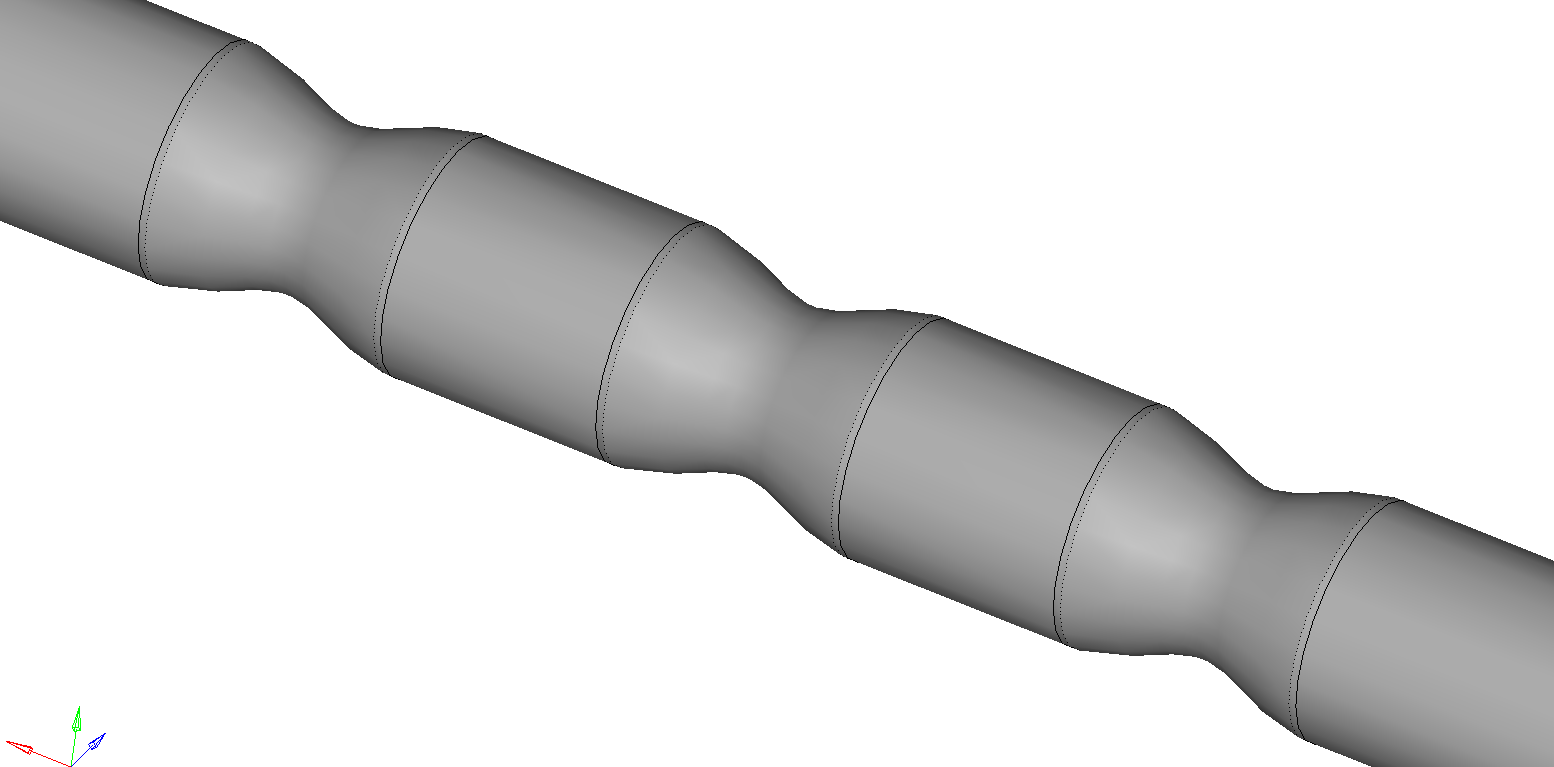
\includegraphics[width=0.6\textwidth]{./pics/geom.png}
	\end{tabular}
	\caption{\footnotesize Geometry of sequential stenoses.}
\end{figure}

\subsection{Mesh}
We implement unstructured hexahedral meshes for idealized stenoses geometry. Internal mesh is total unstructured as the following figure. Moreover, we impose flour boundary layers along the surrounding wall for more accurate prediction of boundary flow.

\begin{figure}[H]
	\centering
	\begin{tabular}{cc}
		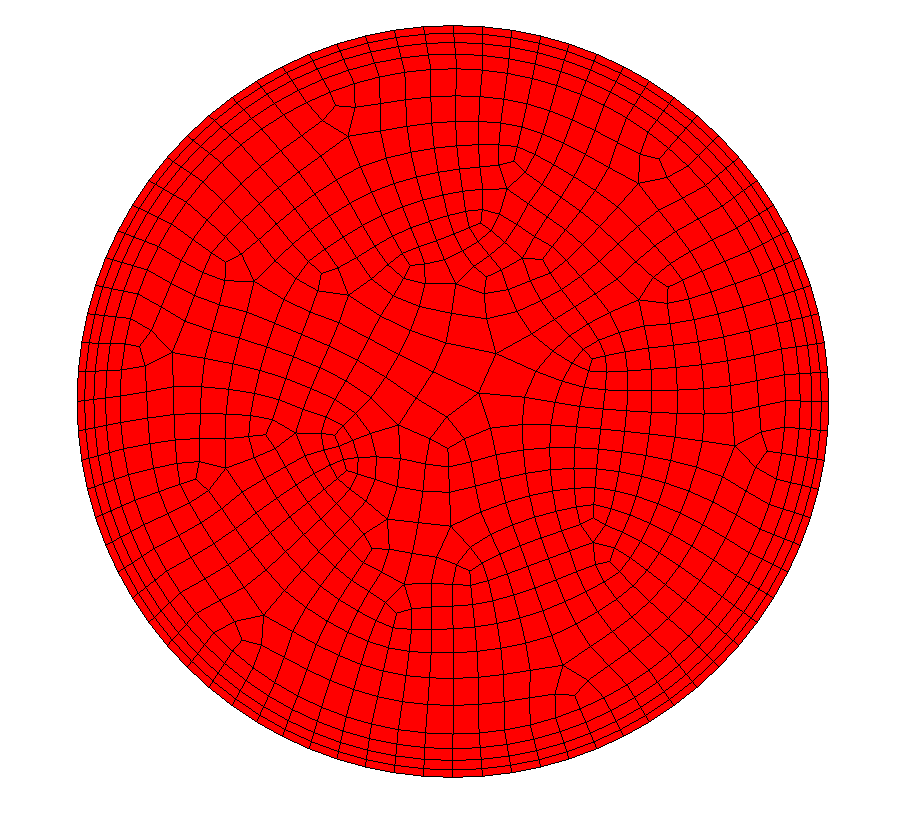
\includegraphics[width=0.3\textwidth]{./pics/mesh1.png} & 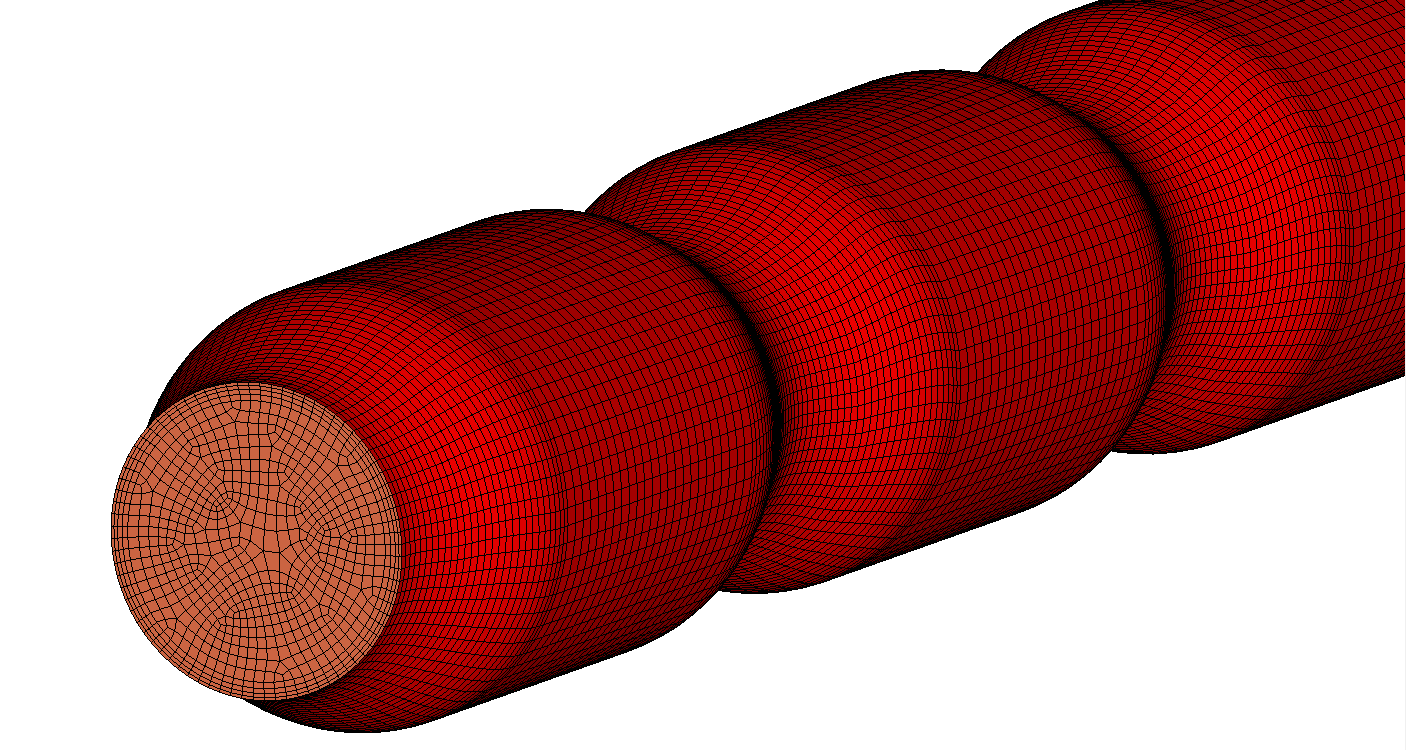
\includegraphics[width=0.6\textwidth]{./pics/mesh7.png}
	\end{tabular}
	\caption{\footnotesize Cross-sectional view of hexahedral meshes.}
\end{figure}

To better analyze the flow cross the stenotic area, we refine the longitudinal mesh across the stnosis. We increase the number of layers along x-axis direction for a better mesh adaptation of stenosis curve.

\begin{figure}[H]
	\centering
	\begin{tabular}{cc}
		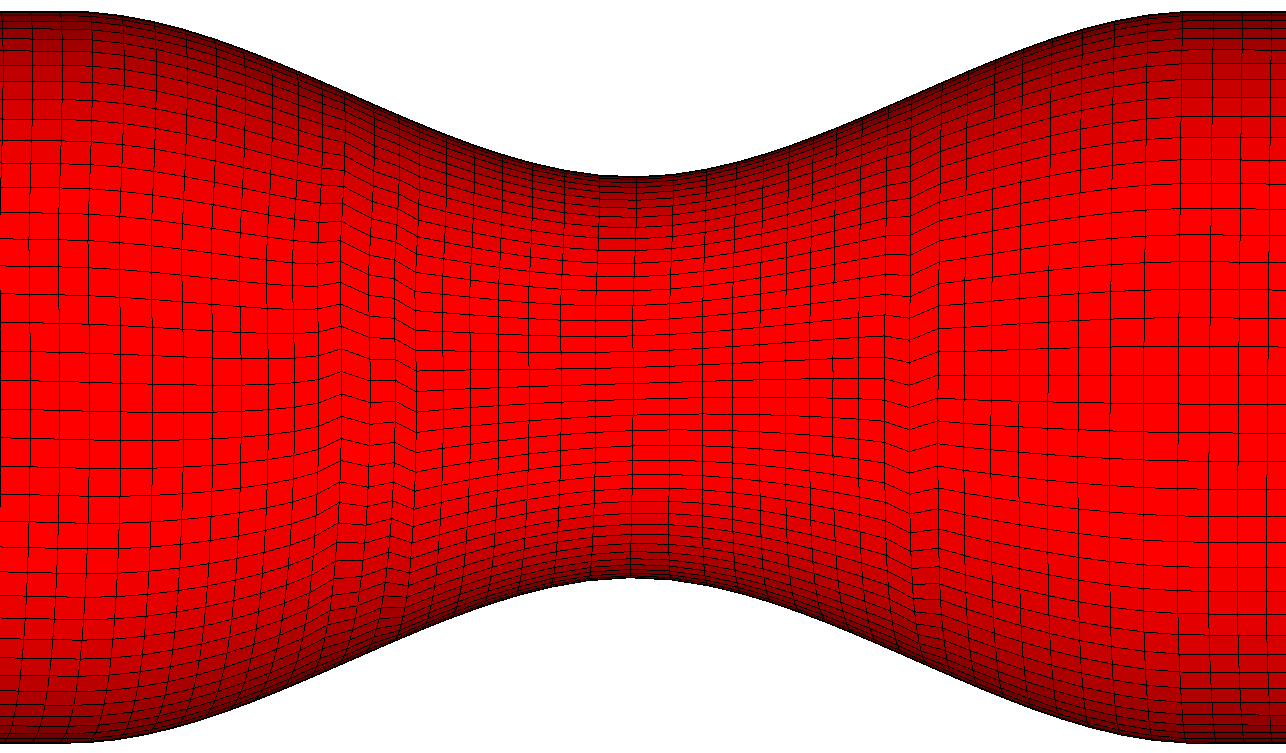
\includegraphics[width=0.4\textwidth]{./pics/refine1.png} & 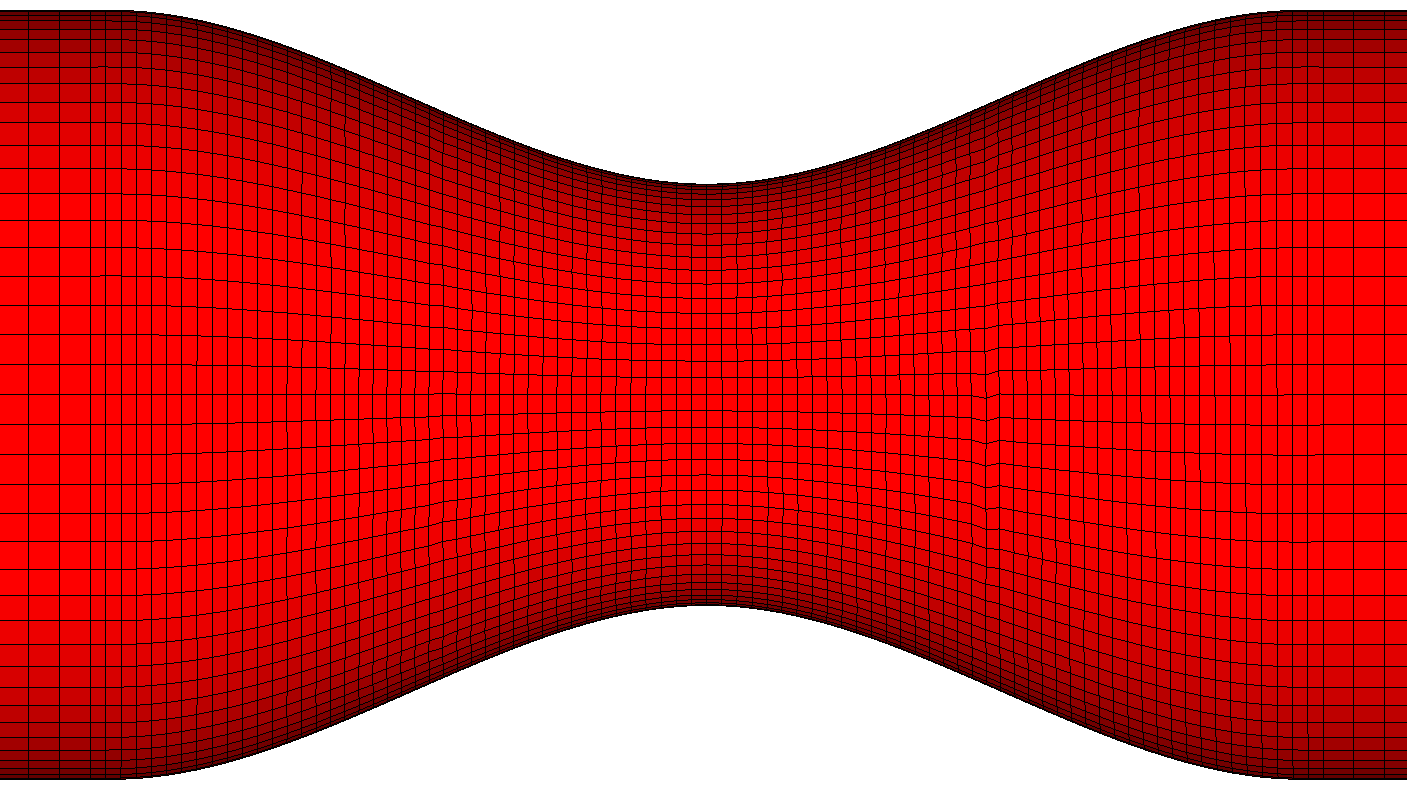
\includegraphics[width=0.4\textwidth]{./pics/refine2.png}
	\end{tabular}
	\caption{\footnotesize Mesh refinement for stenotic area.}
\end{figure}

\subsection{Dimensionless wall distance}

The transition flow happens when the flow passing critical (i.e. $ >70\% $) stenosis. The dimensionless wall distance is defined as:

\begin{equation}
y^{+} = \frac{u_{*} y}{\nu}
\end{equation}

where $u_*$ is the friction velocity at nearest wall, $y$ is the distance to the nearest wall,$\nu$ is the local. kinematic viscosity of fluid. 
We control the $y^+ \le 1$ after refine the mesh with boundary layers. This condition insure that viscosity plays an important role rather than advection.

\subsection{Conditions}

	\begin{table}[!h]
		\caption{ Simulation condition parameters.}
		\vspace{-5pt}
		\begin{center}
			%	\scalebox{0.6}{
			\begin{tabular}{|c|c|}
				\hline
				\textbf{Variable} &\textbf{Value}\\
				\hline
				Stream wise length & 30D\\
				\hline
				Reference mesh points & 720,000\\
				\hline
				Reynolds number for inlet & 500\\
				\hline
				Maximum of CFL number & 0.79\\
				\hline
			\end{tabular}
			%	}
		\end{center} 
	\end{table}

	We implement parabolic velocity profile as inlet boundary condition, Neumann condition as the outlet boundary condition.
	We impose no-slip boundary condition on rigid and non-porous walls.
	The fluid is incompressible Newtonian with same mean Reynolds number as blood in peripheral arteries ${Re}_{mean} = 500$.
	The entrance length of 6 diameters is sufficient for flow development.

%=========================================

\section{Verification}
\subsection{Straight vessel test}
First of all, we implement a simulation on a straight tube without any constriction.
For the straight tube, we use the following analytical function to calculate the pressure drop
\begin{equation}
\Delta P  = \frac{128 \mu l Q}{\pi D^4}
\end{equation} 
We compare the pressure drop between simulation results and analytical solution. The error is less than $0.25$\%.

\begin{table}[h]
	\caption{ Straight vessel test results.}
	\vspace{-5pt}
	\begin{center}
		%	\scalebox{0.6}{
		\begin{tabular}{|c|c|}
			\hline
			\textbf{Cases} &\textbf{Value}\\
			\hline
			Simulation result & 408.6 \\
			\hline
			Analytical solution & 409.9 \\
			\hline
			Error & $<0.25$\% \\
			\hline
		\end{tabular}
		%	}
	\end{center} 
\end{table}

For the following cases, we use the value of pressure drop through the straight tube as a reference bar.
All the parameters including absolute and stream-wise pressure drop are plotted over the reference value.
The coordinate information are plotted over the diameter.
Then all the parameters on the following figures are dimensionless.

\subsection{Resolution independence test}

In this section, we present the results of same geometry with two different mesh resolutions.
The test cases are straight tubes with 10 diameters long. 

\begin{figure}[H]
	\centering
	\begin{tabular}{cc}
		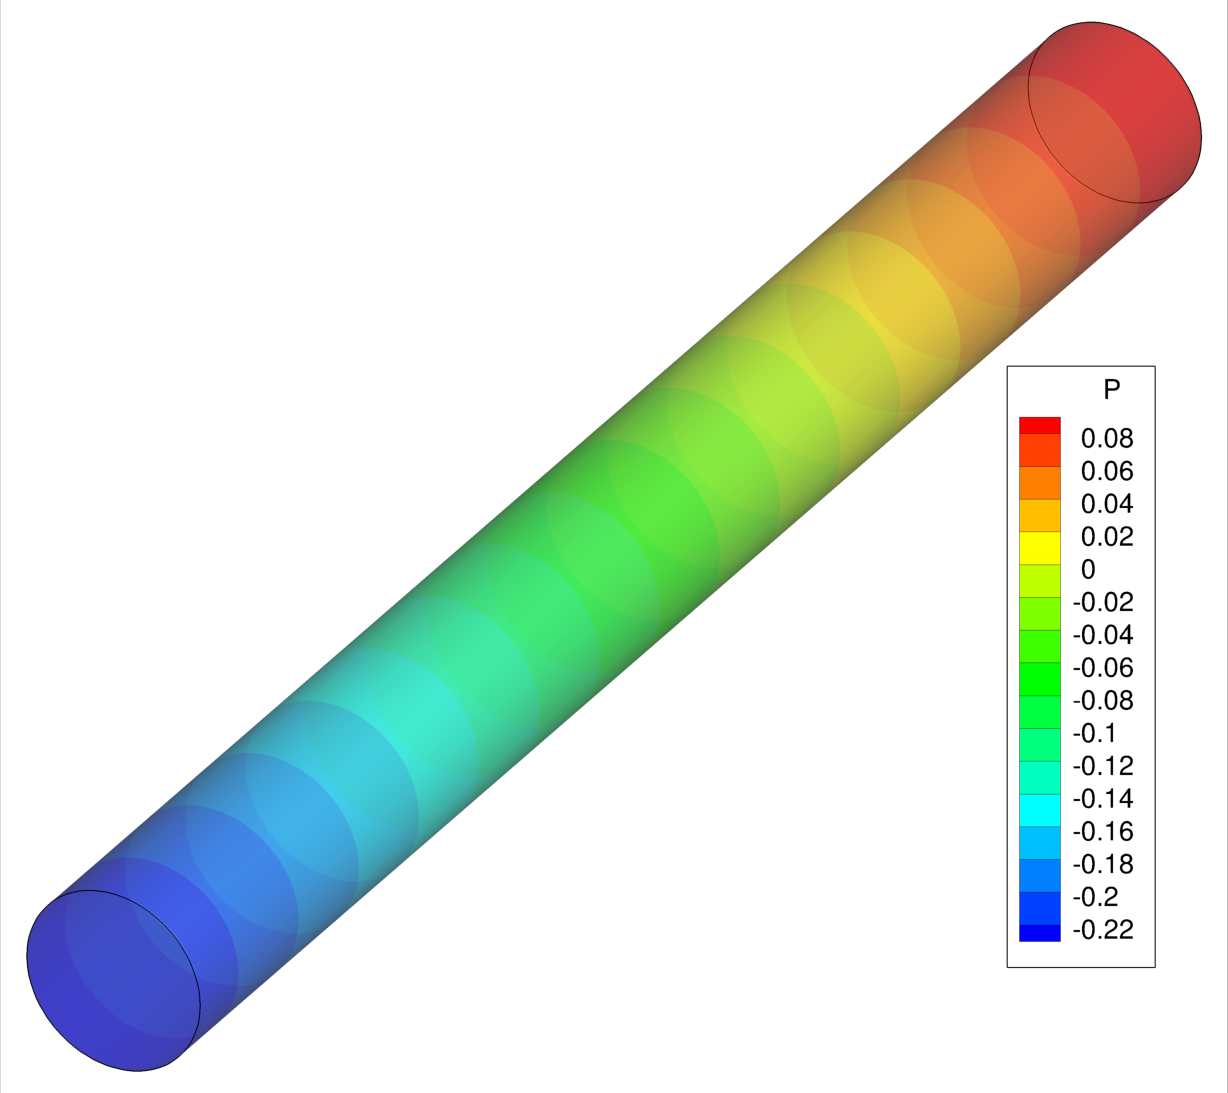
\includegraphics[width=0.4\textwidth]{./pics/plotbio.png} & 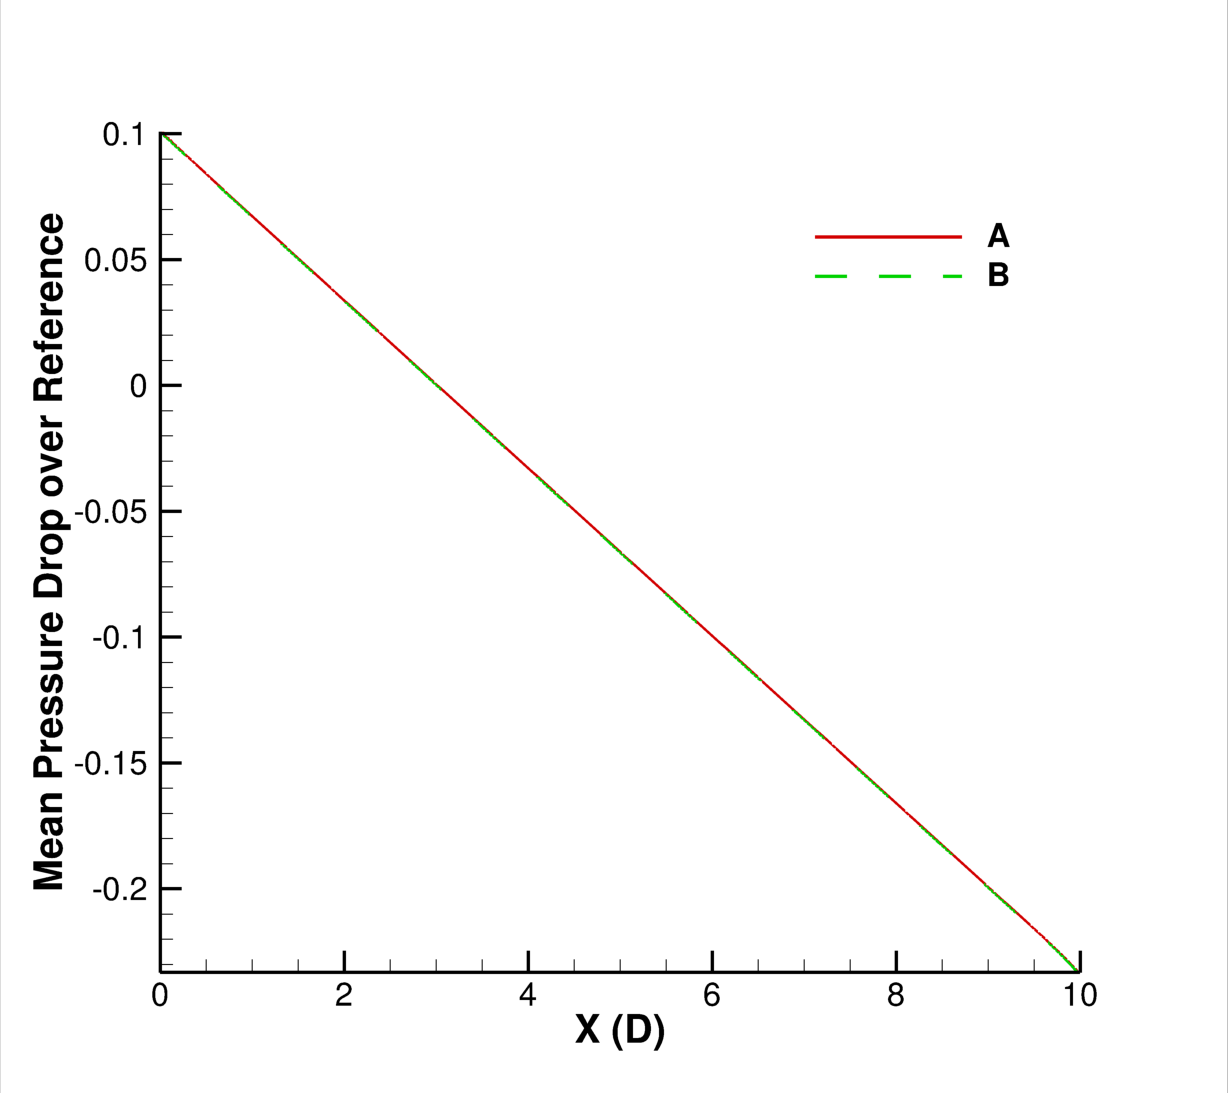
\includegraphics[width=0.4\textwidth]{./pics/resolution.png}
	\end{tabular}
	\caption{\footnotesize Resolution independence test plot and results comparison.}
\end{figure}

The reference mesh grids number of case A is 240000. The resolution of case A is as same as the rest simulations of this paper. We double the number of mesh grid along the longitudinal direction. The finer mesh case B has 480000 grid points. Then we simulate both cases with our solver and compare the results with analytical solution.

\begin{table}[h]
	\caption{Resolution independence test results.}
	\vspace{-5pt}
	\begin{center}
		%	\scalebox{0.6}{
	\begin{tabular}{|c|c|c|}
		\hline
		\textbf{Cases} &\textbf{Value} & \textbf{Error}\\
		\hline
		A & 136.946 & $<0.57\%$\\
		\hline
		B & 137.211 & $<0.76\%$\\
		\hline
		Analytical & 136.169 & 0 \\
		\hline
	\end{tabular}
		%	}
	\end{center} 
\end{table}

The error of both cases are very low and neglectable. The resolution of case A is same as all the simulations in this paper. From this comparison we can conclude that our resolution is sufficient for pipe-flow study. It is a good compromise on accuracy and efficiency of simulations.

%===================================================
\section{Results}

To analyze the hemodynamic effect caused by variant stenoses, we introduced two key parameters which describe the pressure field through stenotic artery. 
The first one is the  stream-wise pressure drop which indicates the pressure difference from the inlet to the outflow area through the whole arterial domain.  
It describes the hemodynamic effect of stenoses among the entire flow domain. The doctors currently are using it as a prime clinical indicator to evaluate blood supplement to downstream bodies. Doctors are using this parameter to make the treatment decision.
The other one is the absolute pressure drop which means the pressure difference between the maximum pressure value (at the inflow area) and minimum pressure value (at the last post-stenotic area). 
This parameter demonstrates the stenotic lesion induces a low pressure field concentrated at the post-stenotic area. 
The certain low pressure flow area is a potential serious damage source to the blood vessels which may leads to restenosis after the treatment. 

\subsection{Verification Empirical Solution}

In Young and Tsai\cite{Young&Tsai} study, the major factors controlling the pressure drop, $\triangle p$, across a single stenosis can be estimated from the following empirical equation:

\begin{equation}
\triangle p = \frac{K_v \mu}{D} U + \frac{K_t}{2}(\frac{A_0}{A_1} -1)^2 \rho \lvert U \rvert U %+ K_u \rho L \frac{dU}{dt}
\end{equation}
where $A_0$ = area of the unobstructed tube, $A_1$ = minimum cross-sectional area of the stenosis,
$D$ = unobstructed tube, $K_v$ and $K_t$ = experimentally determined coefficients, 
$L$ = length over which the pressure drop is measured, $U$ = instantaneous velocity in the unstructed tube,
$\rho$ = blood flow density, and $\mu$ = blood flow viscosity. 

Young et al\cite{Young&Cholvin} pointed out that $K_v$ and $K_t$ are dependent on stenosis geometry and narrowing degree.
$K_v$ can be approximated from steady-flow tests with streamlined plug as single stenosis.
The values of $K_v$ in our simulations range from 630 to 2300 of the stenosis narrowing degree from 40\% to 80\% area reduction.
Another empirical coefficient, $K_u$, gives the best fit of data is 1.2.

\begin{figure}[H]
	\centering
	\begin{tabular}{c}
		\includegraphics[width=0.8\textwidth]{./pics/ana3.png}
	\end{tabular}
	\caption{\footnotesize Pressure drop after single stenosis results from analytic equation and simulation.} \label{fig: single verification}
\end{figure}

In an effort to obtain the theoretic solution, we calculated the pressure drop introduced by single subcritical and critical stneosis with using equation (4).
The parameters including diameters, Reynolds number, viscosity, density and reduction area degrees are all identical for both analytical calculations and computational simulations.
We plot the pressure drop introduced from single stenosis ranges from 40\% to 80\% stenotic narrowing degrees.
The absolute pressure drop marker from simulations are very close to the theoretic calculations. 
The average error between two sets of values are less than 20\%. 


\subsection{Single stenosis evaluation}

\begin{figure}[H]
	\centering
	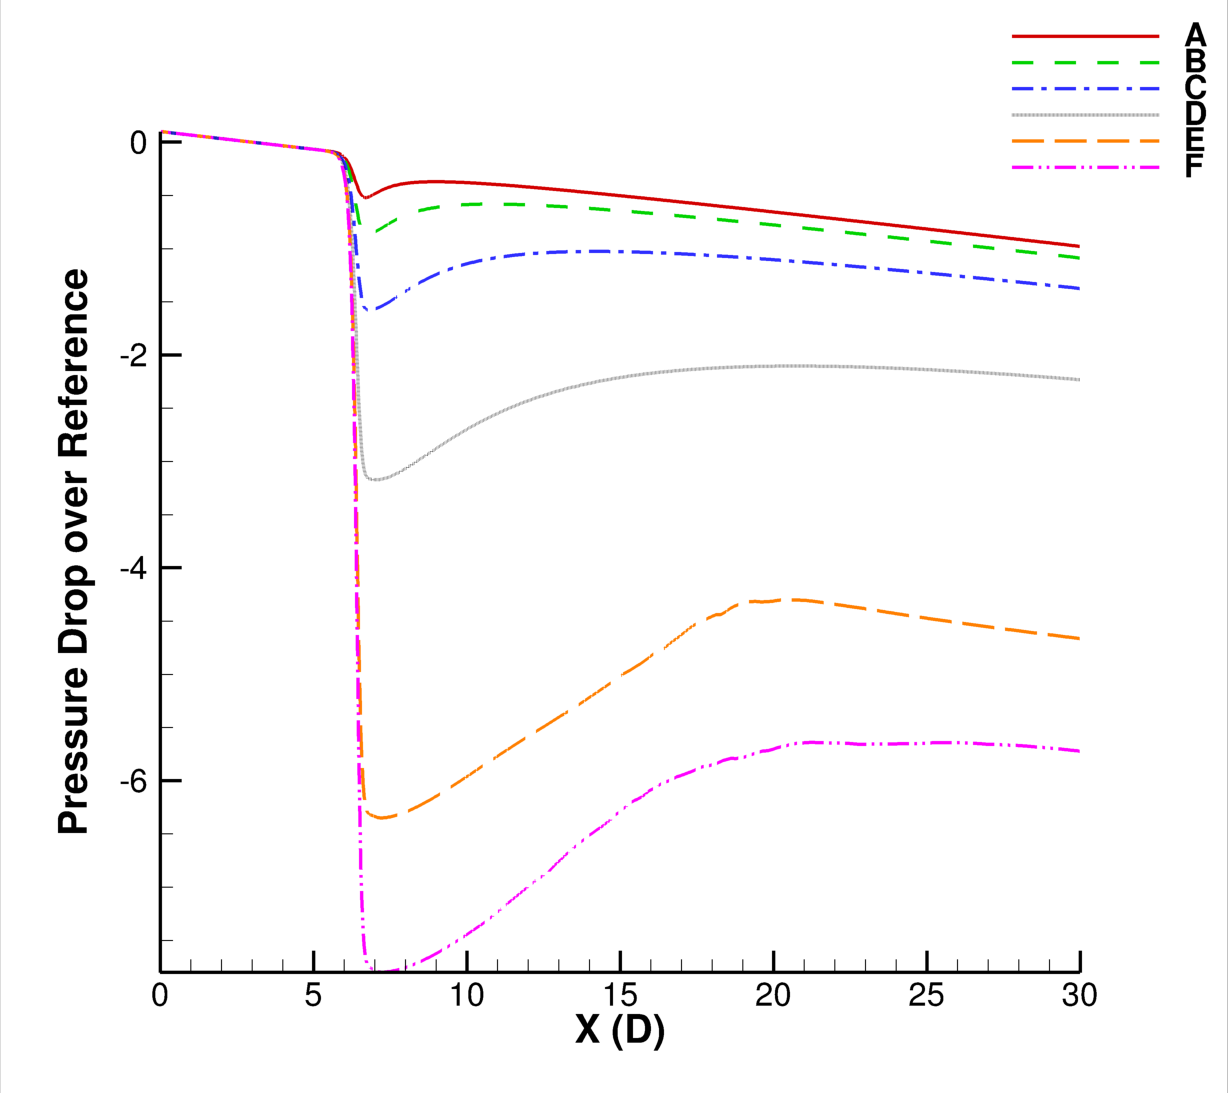
\includegraphics[trim= 1mm 0mm 1mm 0mm,clip,width=0.70\textwidth]{./pics/increase.png}
	\caption{Mean pressure drop of single stenosis for different blocking ratio}
	\label{fig:single increase}
\end{figure}

\begin{table}[h]
	\caption{Mean pressure drop of single stenosis for different blocking ratio}
	\vspace{-5pt}
	\begin{center}
		%	\scalebox{0.6}{
		\begin{tabular}{|c|c|c|c|}
			\hline
			\textbf{Cases} &\textbf{Degree} & \textbf{Streamwise PD} & \textbf{Absolute PD}\\
			\hline
			A & 40\% & 1.080 & 0.622\\
			\hline
			B & 50\% & 1.089 & 0.975\\
			\hline
			C & 60\% & 1.476 & 2.027\\
			\hline
			D & 70\% & 2.437 & 3.897\\
			\hline
			E & 78\% & 4.766 & 7.543\\
			\hline
			F & 80\% & 5.823 & 9.184\\
			\hline
		\end{tabular}
		%	}
	\end{center} 
\end{table}
